%Set document format
\documentclass[11pt]{article}
\usepackage[margin=1in]{geometry}

%Set up packages
\usepackage{amsmath,amssymb,amsthm}
\usepackage{graphicx}
\usepackage{textcomp, gensymb}
\usepackage{float}
\usepackage{pdfpages}
\usepackage[hidelinks]{hyperref}
\usepackage{cancel}
\usepackage{subcaption}
\usepackage{caption}
 
\newcommand{\bm}{\boldsymbol}
\newcommand{\bI}{\mathbb{I}}
\newcommand{\bR}{\mathbb{R}}

\setlength\parindent{0pt}


\title{\bf OF-1 Report : \\[2mm] Computational Simulations of a Lid-driven Cavity}
\author{Terry Murray (tnm3843), Nicole Olvera (no4342), Andres Suniaga (aas5778)}
\date{02/11/2025}

\begin{document}
\maketitle

\noindent\makebox[\textwidth]{\rule{\textwidth}{0.2pt}}
\tableofcontents
\noindent\makebox[\textwidth]{\rule{\textwidth}{0.2pt}}
\pagebreak

\section{Introduction}
This report invesitages the canonical case of CFD, a lid-driven cavity. The \textit{OpenFOAM} software is used to compute the velocity and pressure fields at a given Reynolds number, which is the sole non-dimensional property that dictates the flow for the cavity. Thus we consider the nondimensionalized form of the incompressible, steady Navier-Stokes equations. \textit{Paraview} software is used for visualizations of the velocity and pressure fields of the cavity which are included in the report.
\vspace{2.5mm}

Experiments between different mesh refinments and Reynolds numbers are conducted to show changes in velocity fields, nondimensionalized shear stresses, nondimensionalized forces, and the execution or \textit{wallclock} time per step of each refinement. 


% The incompressible \& steady form of the Navier-Stokes equations is considered for the case of a 2-D lid-driven cavity with height = $H$, length = $L$, and lid velocity = $U$. The non-dimensional forms of the continuity and momentum equations are recorded. After visualizing the solution for Re = 10, we experiment with the size of the grid to compare \textit{wallclock} or execution times with the refined solutions. We then estimate the relationship between \textit{wallclock} time and the total number of grid points. We compute and plot the non-dimensional shear stress along the lid at a few Reynolds numbers between 10 and 500. Finally, we compute the resulting force on the lid aspect ratios 1/2, 1, and 2 and Reynolds numbers between 10 and 500. "TBR"


\section{Nondimensional Navier-Stokes equations}
The incompressible, constant density, $\rho$, and viscocity, $\mu$, steady form of the Navier-Stokes equations govern the prescribed two-dimensional fluid flow problem. The continuity and momentum equations are non-dimensionalized according to the following scales:
\begin{itemize}
    \item Length scale L = $\dfrac{x}{\tilde{x}}$ = $\dfrac{y}{\tilde{y}}$
    \item Velocity scale U = $\dfrac{u}{\tilde{u}}$ = $\dfrac{v}{\tilde{v}}$
    \item Pressure Scale $\tilde{P}$ = $\dfrac{P}{\rho U^2}$
    \item Reynolds number Re = $\dfrac{\rho UL}{\mu} = \dfrac{UL}{\nu}$ where $\nu = \mu/\rho$ is the kinematic viscocity
\end{itemize}

\subsection*{Continuity}
\begin{equation*}
    \frac{\partial \tilde{u}}{\partial \tilde{x}} + \frac{\partial \tilde{v}}{\partial \tilde{y}} = 0
\end{equation*}

\subsection*{X-Momentum}
\begin{equation*}
    \tilde{u} \frac{\partial \tilde{u}}{\partial \tilde{x}} + \tilde{v} \frac{\partial \tilde{u}}{\partial \tilde{y}} = -\frac{\partial \tilde{p}}{\partial \tilde{x}} + \frac{1}{Re}\left(\frac{\partial^2 \tilde{u}}{\partial \tilde{x}^2} + \frac{\partial^2 \tilde{u}}{\partial \tilde{y}^2}\right)
\end{equation*}

\subsection*{Y-Momentum}
\begin{equation*}
    \tilde{u} \frac{\partial \tilde{v}}{\partial \tilde{x}} + \tilde{v} \frac{\partial \tilde{v}}{\partial \tilde{y}} = -\frac{\partial \tilde{p}}{\partial \tilde{y}} + \frac{1}{Re}\left(\frac{\partial^2 \tilde{v}}{\partial \tilde{x}^2} + \frac{\partial^2 \tilde{v}}{\partial \tilde{y}^2}\right)
\end{equation*}
\vspace{2.5mm} 

In the momentum equations, the only non-dimensional number that appears is the Reynolds number. When the Reynolds number becomes very large ($Re \rightarrow \infty$), the viscous terms on the RHS of the equations become negligible, implying inviscid flow, reducing the momentum equations to the Euler equations. When the Reynolds number becomes very small ($Re \rightarrow 0$), the viscous terms on the RHS of the equations become very large, implying a highly viscous flow, reducing the momentum equations to the Stokes equations. The Stokes and Euler equations are listed below. 
\vspace{5mm}

\subsection*{Euler Equations:}

\vspace{5mm}

\textbf{Continuity as $Re \rightarrow \infty$:}
\begin{equation*}
\frac{\partial \tilde{u}}{\partial \tilde{x}} + \frac{\partial \tilde{v}}{\partial \tilde{y}} = 0
\end{equation*}

\vspace{2.5mm}

\textbf{X-Momentum as $Re \rightarrow \infty$:}
\[
\tilde{u} \frac{\partial \tilde{u}}{\partial \tilde{x}} + \tilde{v} \frac{\partial \tilde{u}}{\partial \tilde{y}} = -\frac{\partial \tilde{p}}{\partial \tilde{x}}
\]

\vspace{2.5mm}

\textbf{Y-Momentum as $Re \rightarrow \infty$:}
\[
\tilde{u} \frac{\partial \tilde{v}}{\partial \tilde{x}} + \tilde{v} \frac{\partial \tilde{v}}{\partial \tilde{y}} = -\frac{\partial \tilde{p}}{\partial \tilde{y}}
\]

\vspace{5mm}

\subsection*{Stokes Equations:}


\vspace{5mm}

\textbf{Continuity as $Re \rightarrow 0$:}
\[
\frac{\partial \tilde{u}}{\partial \tilde{x}} + \frac{\partial \tilde{v}}{\partial \tilde{y}} = 0
\]

\vspace{2.5mm}

\textbf{X-Momentum as $Re \rightarrow 0$:}
\[
0 = -\frac{\partial \tilde{p}}{\partial \tilde{x}} + \frac{1}{Re} \left( \frac{\partial^2 \tilde{u}}{\partial \tilde{x}^2} + \frac{\partial^2 \tilde{u}}{\partial \tilde{y}^2} \right)
\]

\vspace{2.5mm}

\textbf{Y-Momentum as $Re \rightarrow 0$:}
\[
0 = -\frac{\partial \tilde{p}}{\partial \tilde{y}} + \frac{1}{Re} \left( \frac{\partial^2 \tilde{v}}{\partial \tilde{x}^2} + \frac{\partial^2 \tilde{v}}{\partial \tilde{y}^2} \right)
\]


\pagebreak



\section{Flow at Re = 10}

\subsection{Plots of Velocity}
\begin{figure}[H]
   \centering
   \begin{subfigure}{0.495\linewidth}
      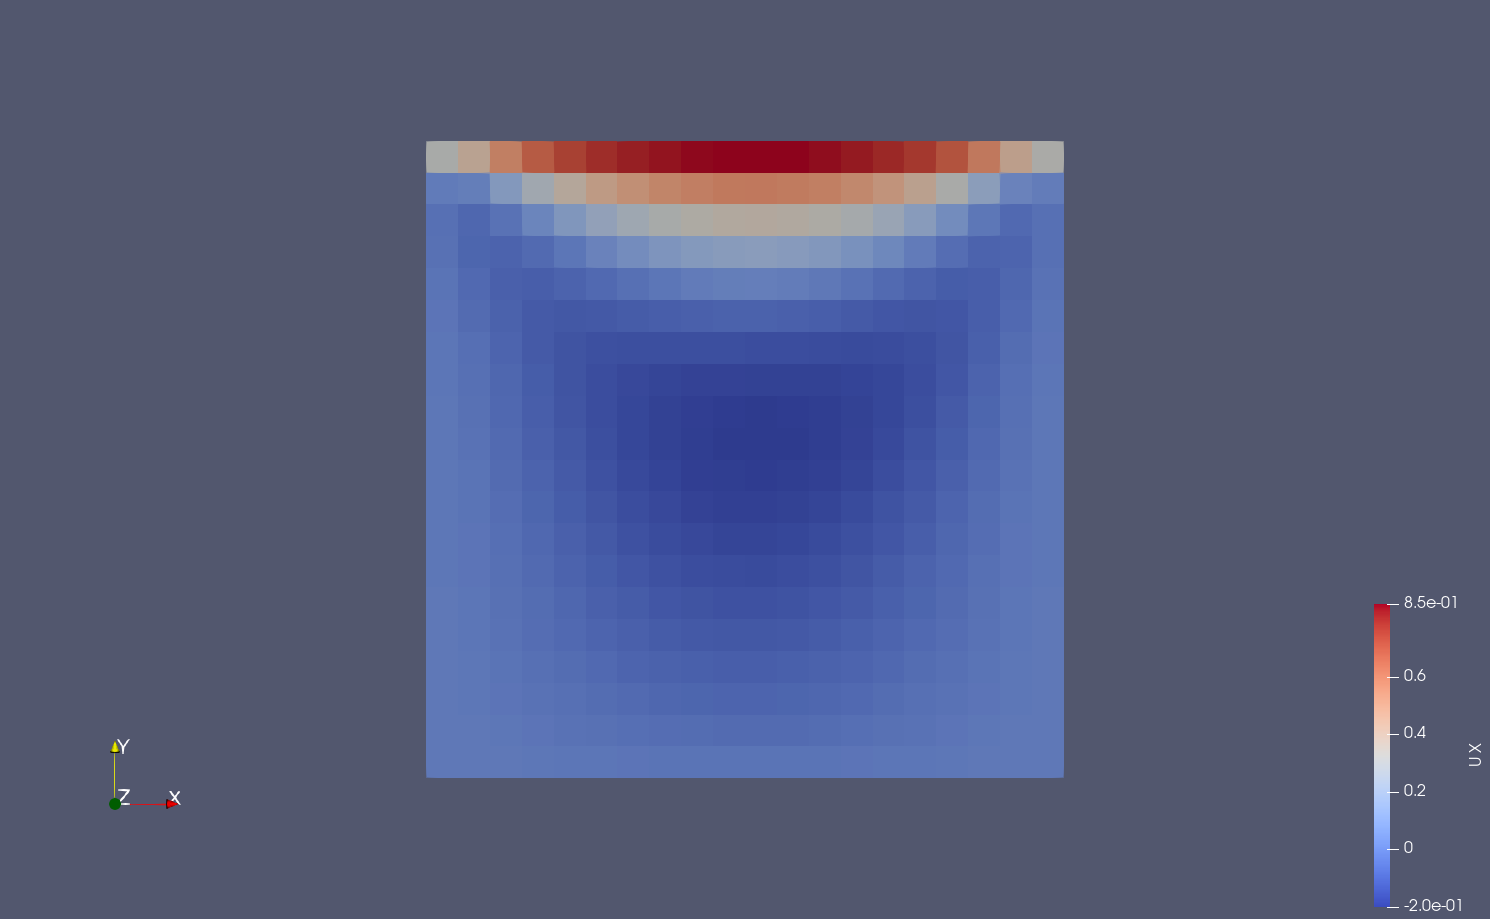
\includegraphics[width=\textwidth]{images/ux_paraview.png}
      \caption{Plot from Paraview of $u$}
   \end{subfigure}
   \begin{subfigure}{0.495\linewidth}
      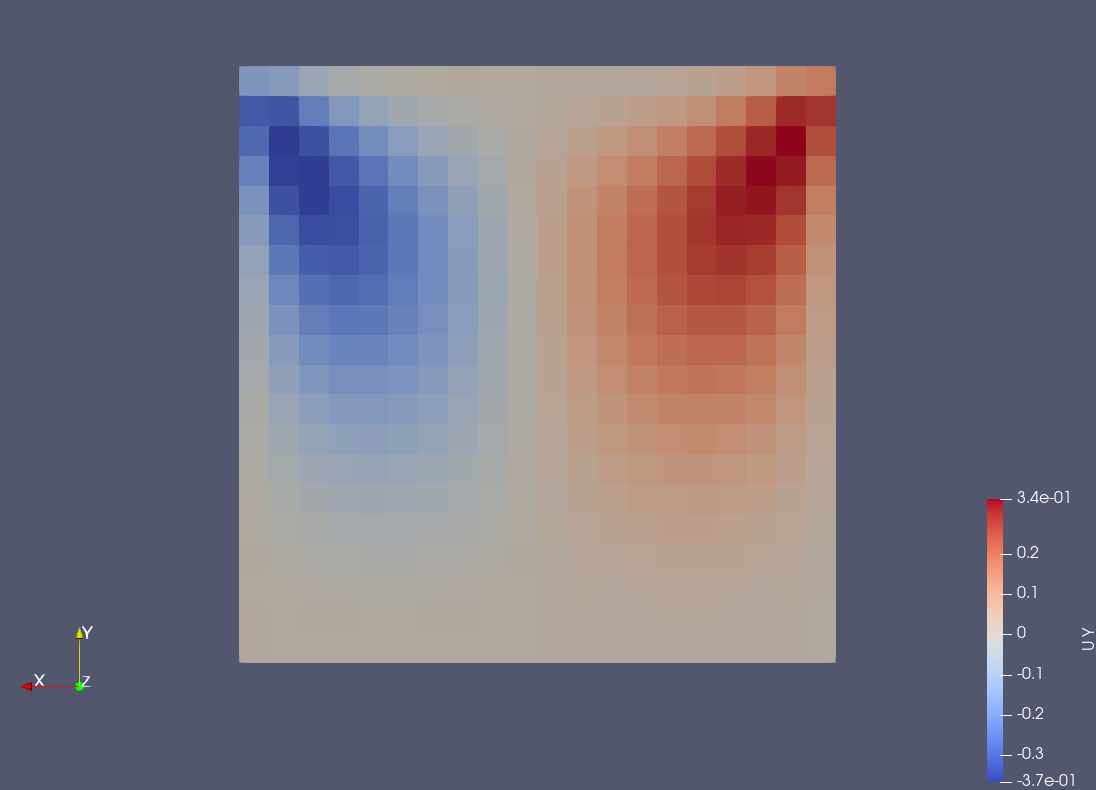
\includegraphics[width=\textwidth]{images/uy_paraview.png}
      \caption{Plot from Paraview of $v$}
   \end{subfigure}      
   \label{paraviewplots}
\end{figure}

\begin{figure}[H]
   \centering
   \begin{subfigure}{0.495\linewidth}
      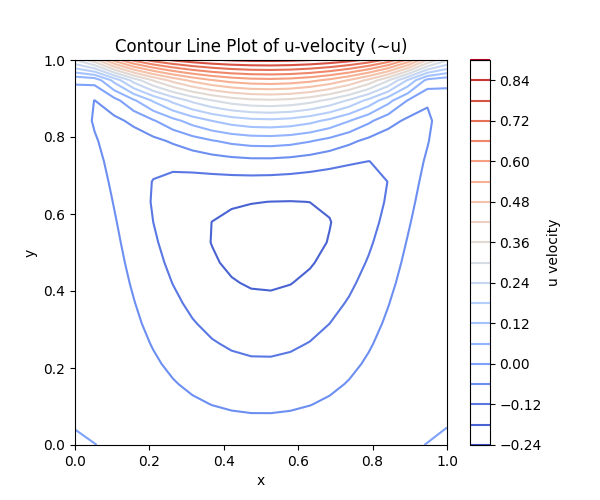
\includegraphics[width=\textwidth]{images/u_velocity.png}
      \caption{Contour Plot of $u/U$}
   \end{subfigure}
   \begin{subfigure}{0.495\linewidth}
      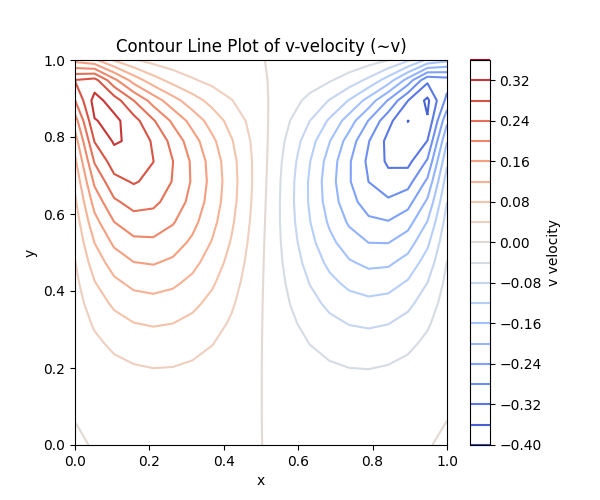
\includegraphics[width=\textwidth]{images/v_velocity.png}
      \caption{Contour Plot of $v/U$}
   \end{subfigure}      
   \label{contourplots}
\end{figure}

\begin{figure}[H]
   \centering
   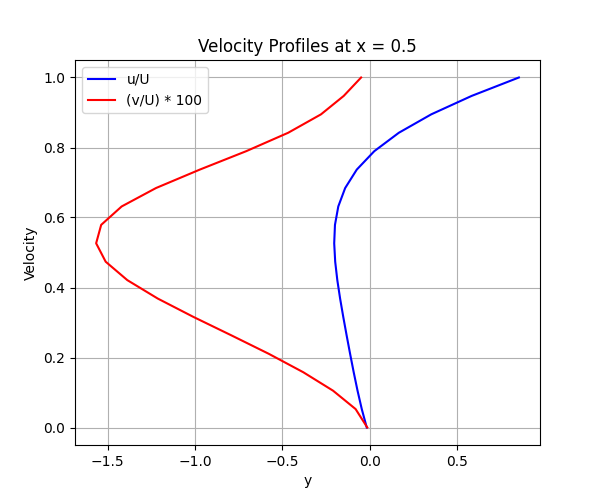
\includegraphics[width=0.65\textwidth]{images/center_velocity.png}
   \caption{$u/U$ and $v/U$ through the center of the cavity}
   \label{originaluv}
\end{figure}

\subsection{Solution Refinement}
\begin{figure}[H]
   \centering
   \begin{subfigure}{0.495\linewidth}
      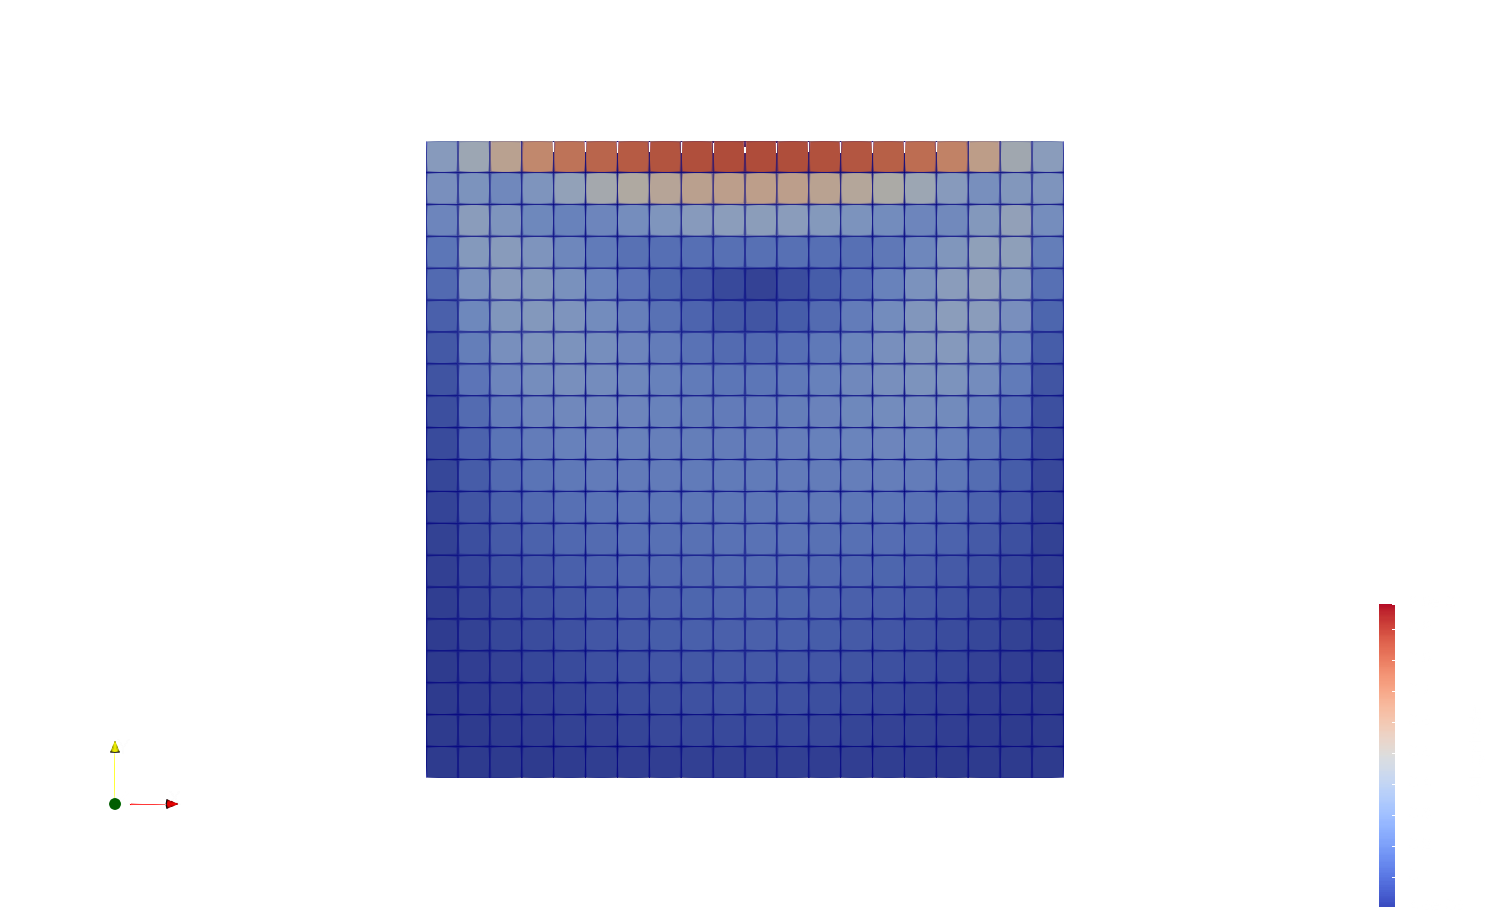
\includegraphics[width=\linewidth]{images/paraview_U_20.png}
      \caption{$N = 20 \times 20$}
   \end{subfigure}
   \begin{subfigure}{0.495\linewidth}
      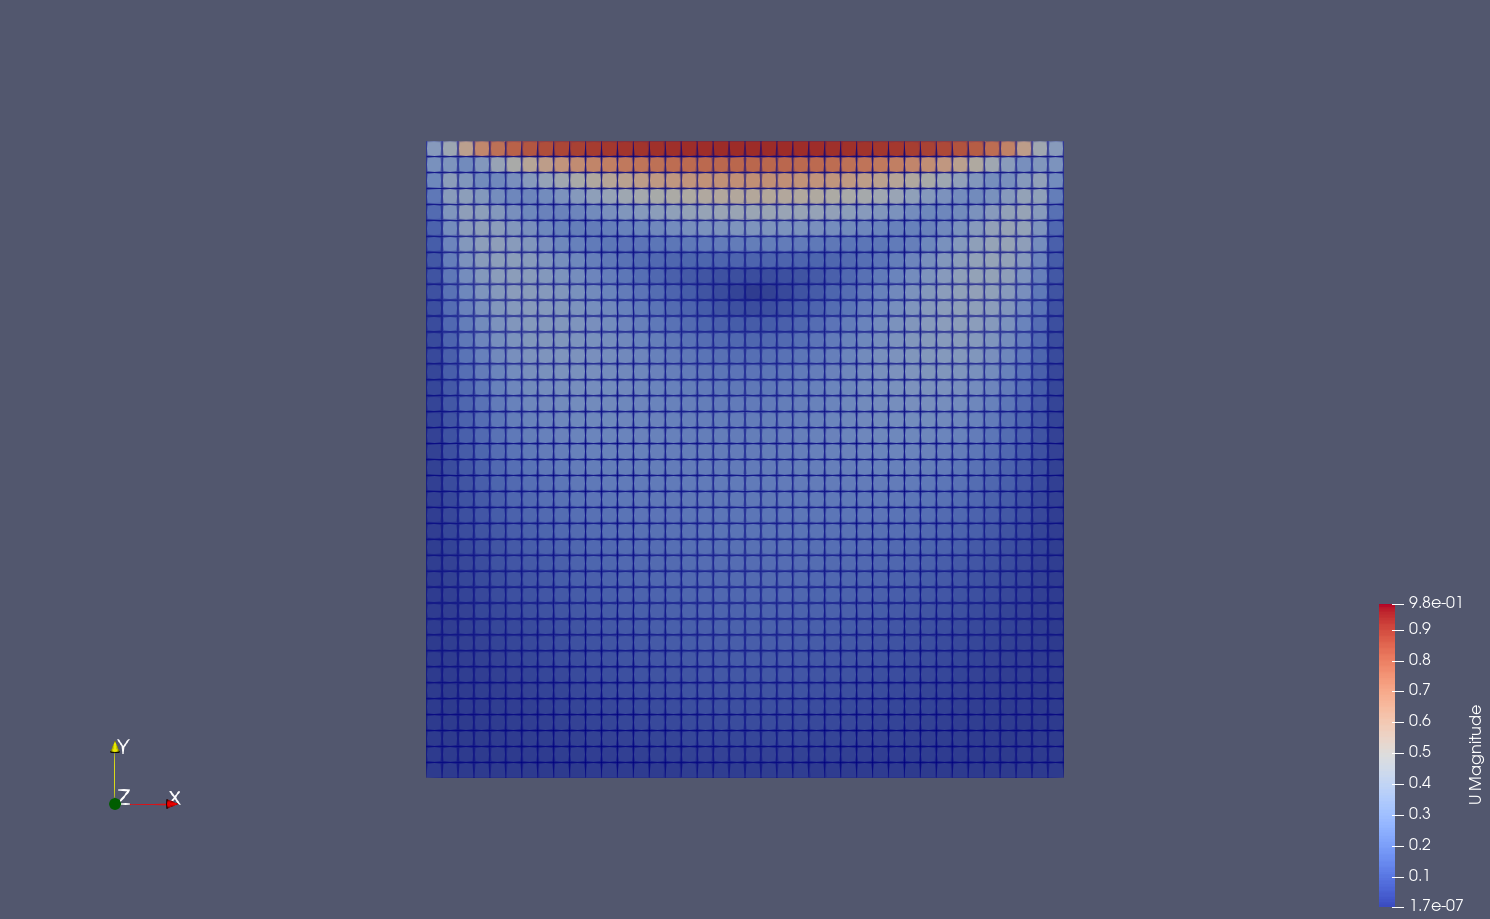
\includegraphics[width=\linewidth]{images/paraview_U_40.png}
      \caption{$N = 40 \times 40$}
   \end{subfigure}
   \vspace{5mm}

   \begin{subfigure}{0.495\linewidth}
      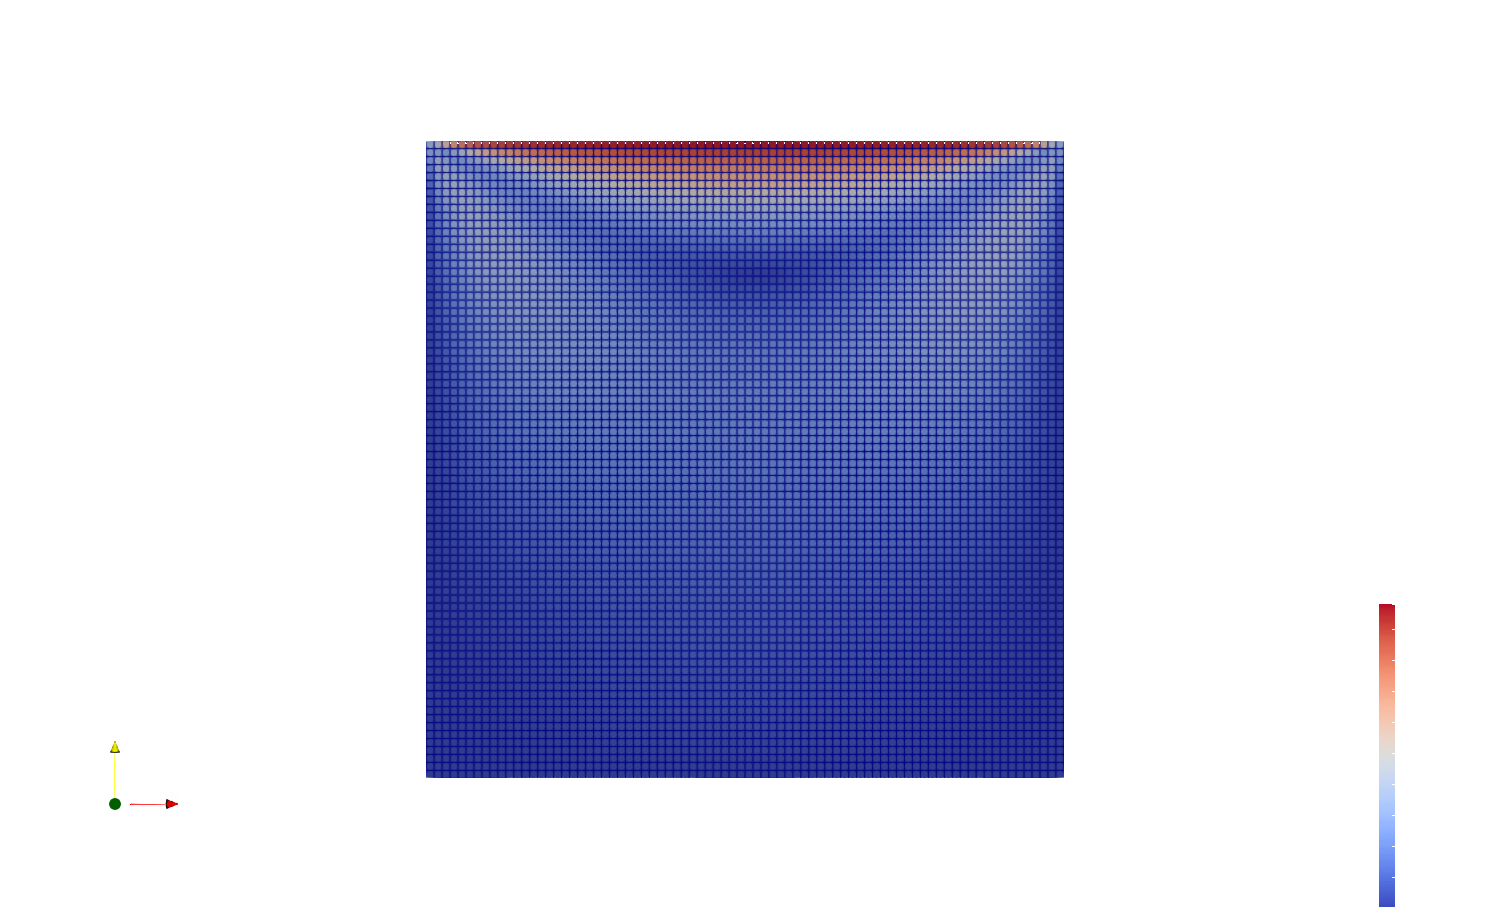
\includegraphics[width=\linewidth]{images/paraview_U_80.png}
      \caption{$N = 80 \times 80$}
   \end{subfigure}
   \begin{subfigure}{0.495\linewidth}
      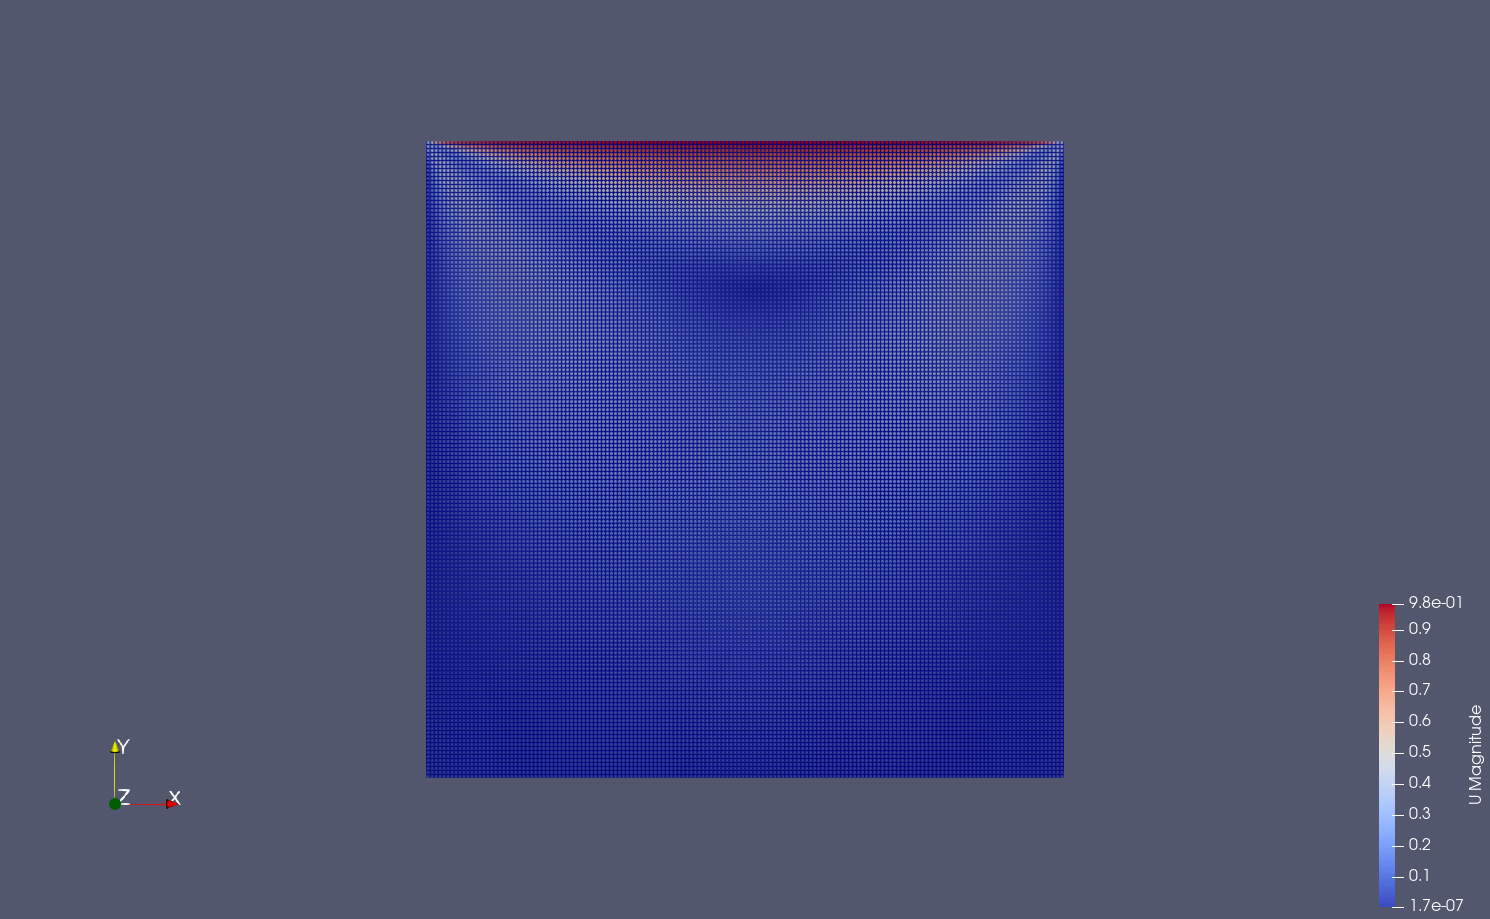
\includegraphics[width=\linewidth]{images/paraview_U_160.png}
      \caption{$N = 160 \times 160$}
   \end{subfigure}
   \caption{Visualizing effect of gridpoint refinement on $U$ in \textit{Paraview}}
   \label{paraviewrefine}
\end{figure}
   

\begin{figure}[H]
   \centering
   \begin{subfigure}{0.495\linewidth}
      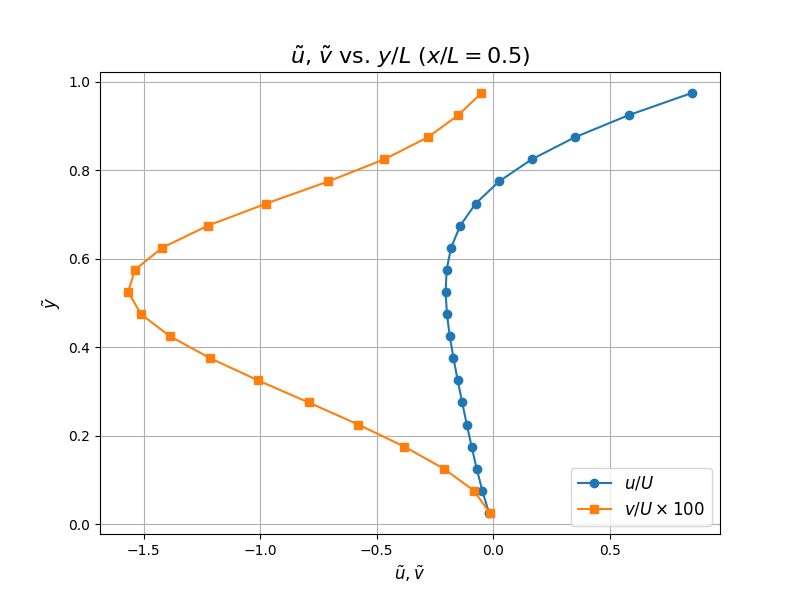
\includegraphics[width=\textwidth]{images/Velocity_Component_Plot_for_gridsize_20x20.png}
      \caption{Original}
   \end{subfigure}
   \begin{subfigure}{0.495\linewidth}
      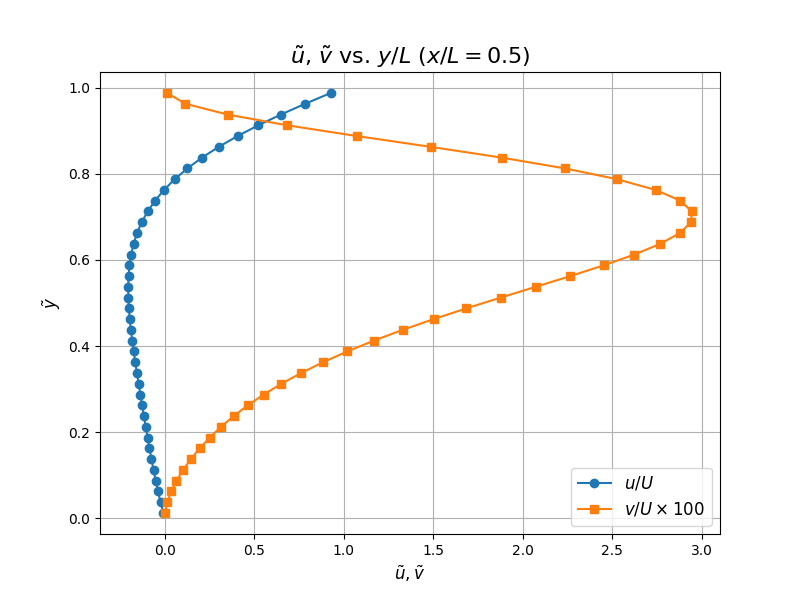
\includegraphics[width=\textwidth]{images/Velocity_Component_Plot_for_gridsize_40x40.png}
      \caption{First Refinement}
   \end{subfigure}
   \vspace{5mm}

   \begin{subfigure}{0.495\linewidth}
      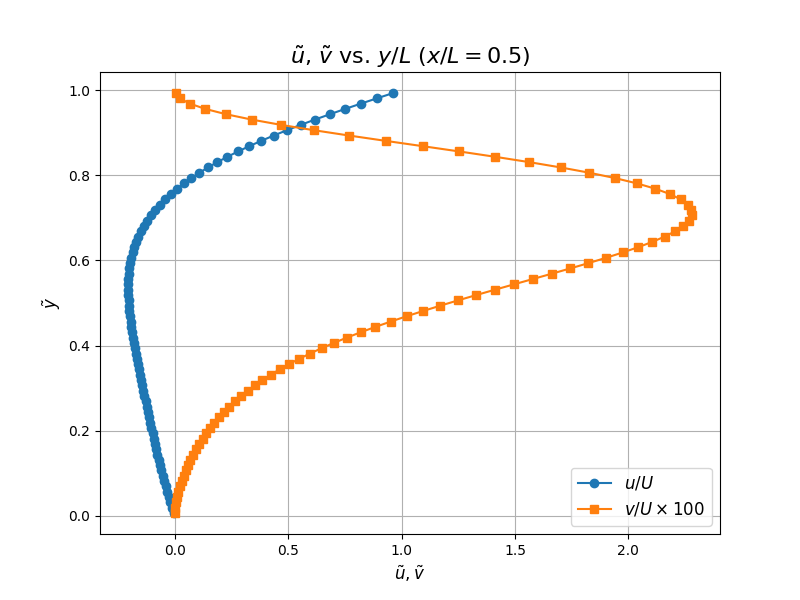
\includegraphics[width=\textwidth]{images/Velocity_Component_Plot_for_gridsize_80x80.png}
      \caption{Third Refinement}
   \end{subfigure}
   \begin{subfigure}{0.495\linewidth}
      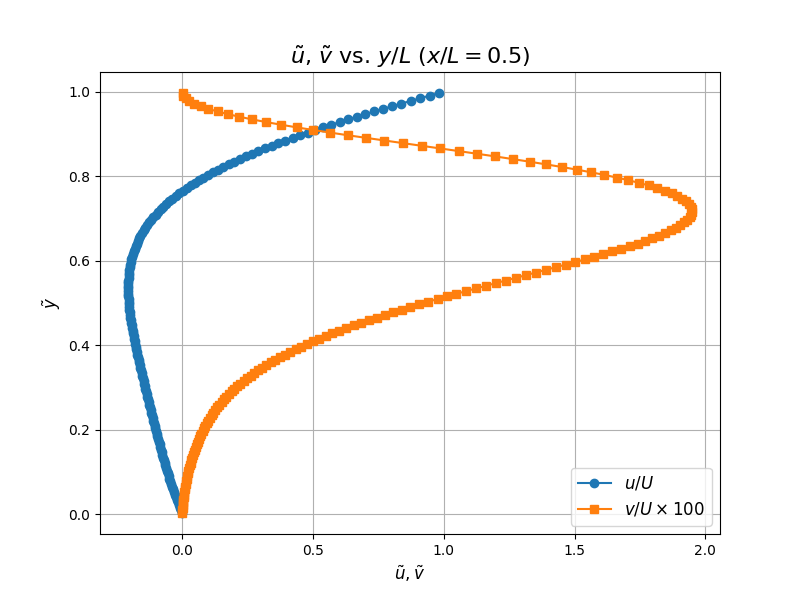
\includegraphics[width=\textwidth]{images/Velocity_Component_Plot_for_gridsize_160x160.png}
      \caption{Fourth Refinement}
   \end{subfigure}
   \vspace{2.5mm}

   \caption{Effect of increased gridsize and decreased time step size on $\tilde{u}$, $\tilde{v}$ vs. $\tilde{y}$}
   \label{velocityrefine}
\end{figure}

There is a noticable variation in the scaled up y-component of $\textbf{U}$ as we refine the mesh further. The x-component of $\textbf{U}$ seems to curve more and reach closer to $u/U = 1$ at $\tilde{y}=1$ as the mesh is futher refined too. 

\pagebreak
\begin{figure}[H]
   \centering
   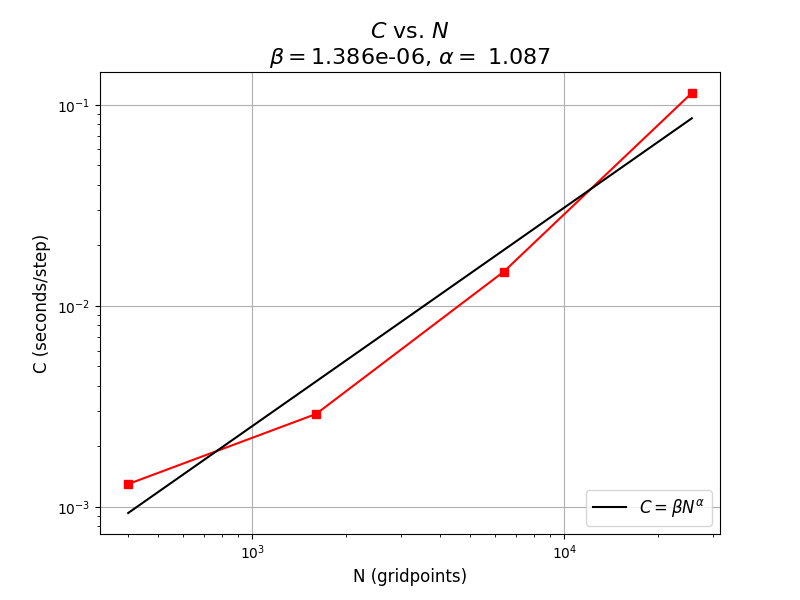
\includegraphics[width=0.85\textwidth]{images/Refinement_Measure.png}
   \caption{Execution time per step $C$ increases with higher gridpoints $N$}
   \label{timerefine}
\end{figure} 

\begin{center} 
   \fbox{\begin{minipage}{0.9\textwidth}
      \textbf{Q:} What can you conclude about the increase in wallclock time as you refine the grid?
   \end{minipage}}
\end{center}

\textbf{A:} Higher refinement will take longer per iteration than at lower refinement. It is clear in Fig. \ref{timerefine} with our estimate of $\alpha = 1.087$ in the fit $C = \beta N^{\alpha}$ that with an order of magnitude increase in gridpoints there is an order of magnitude increase in the execution time per step.

\pagebreak

\section{Force on the Lid}
Now we want to investigate the dependance of the force on Reynolds number. We define a few nondimensionalized terms, I love you andres
\begin{itemize}
   \item $\tilde{F} = \dfrac{F}{\mu U} = \displaystyle \int_{0}^{1} \tilde{\tau}(\tilde{x})\, d\tilde{x}$
   \vspace{2.5mm}

   \item $\tilde{\tau} = \dfrac{\tau L}{\mu U} = \dfrac{\partial\tilde{u}}{\partial\tilde{y}}$
\end{itemize}

With these terms and our solution for Re = 10 (using the 80x80 grid), we generate a plot $\tilde{\tau}$ vs. $\tilde{x}$:
\begin{figure}[H]
   \centering
   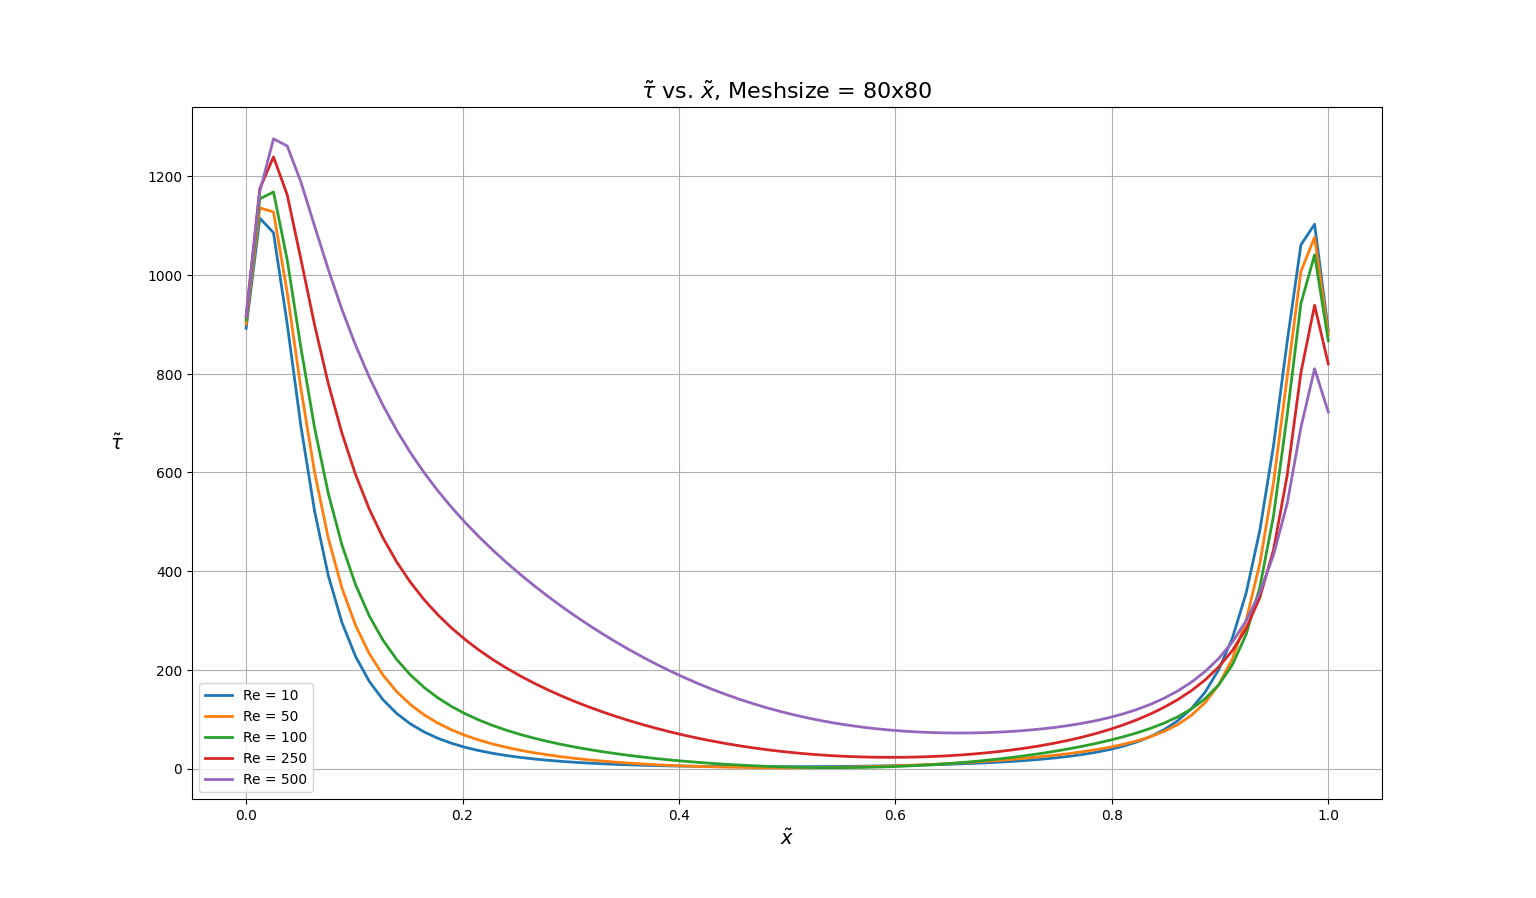
\includegraphics[width = \textwidth]{images/Nondimensional_Stress_vs._x.png}
   \caption{Shear stress has a major decrease over the center of the cavity}
   \label{shear}
\end{figure}

\begin{figure}[H]
   \centering
   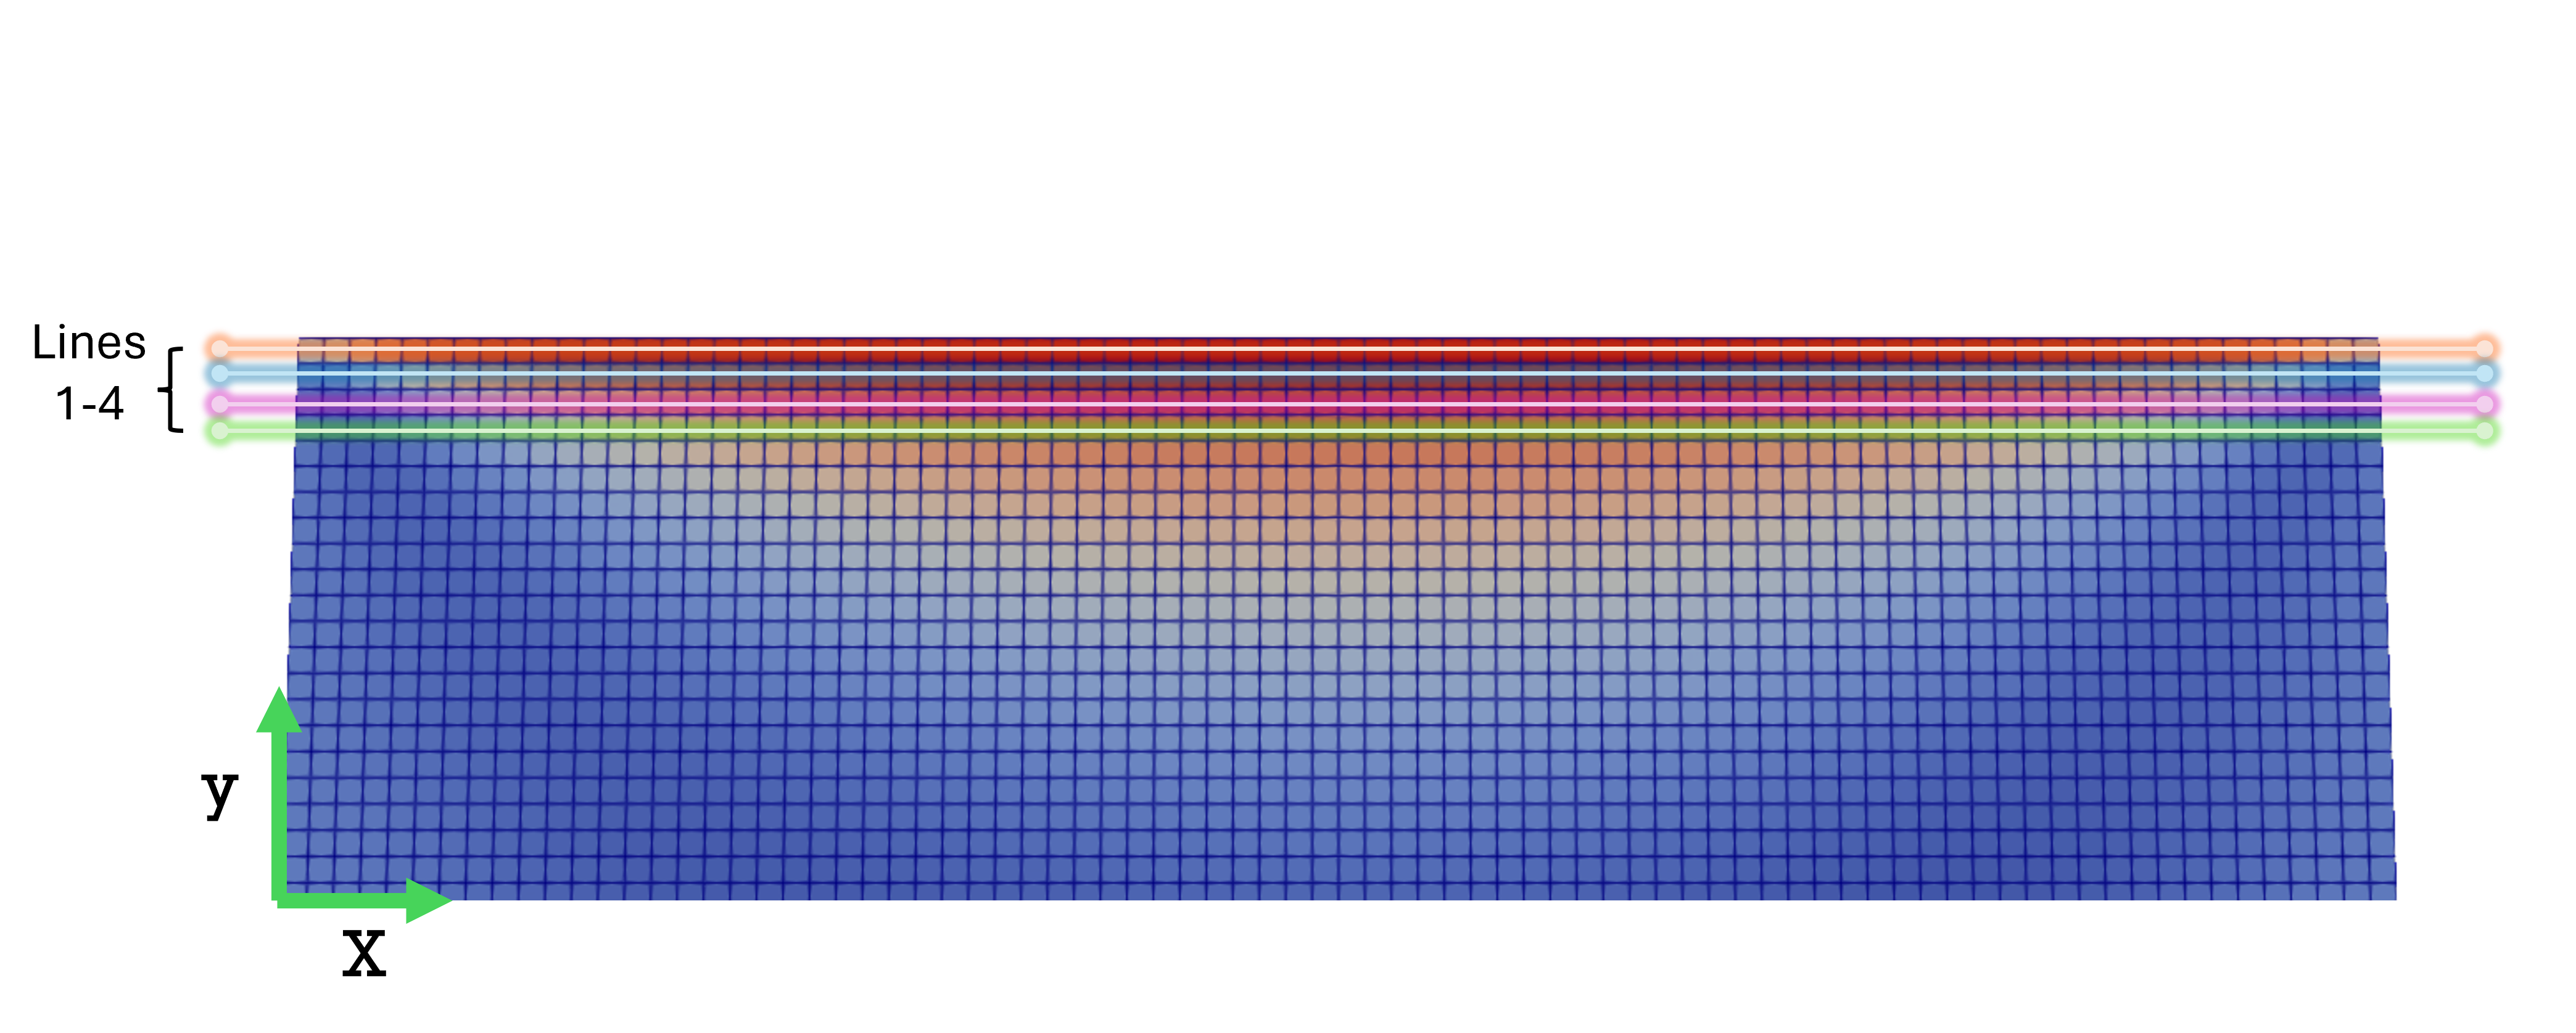
\includegraphics[width = 0.8\textwidth]{images/80mesh_extractingstress.png}
   \caption{Extracting shear stress through polynomial fitting on top $4$ rows $80$x$80$ Mesh}
   \label{80meshstress}
\end{figure}

To obtain the nondimensionalized shear stress curves as shown in Fig. \ref{shear}, we fit a second-order polynomial as a function of $y$ through the first four rows of the $80$x$80$ grid as seen in Fig. \ref{80meshstress}. That is,
\begin{equation*}
   u_{i}(y) = a_{i}y^{2} + b_{i}y + c_{i}
\end{equation*}
\vspace{1mm}

where $i$ is the gridpoint $1$ to $80$ along the line. Recall $\tilde{\tau} = \dfrac{\partial\tilde{u}}{\partial\tilde{y}}$. We obtain $\tilde{\tau}$ on the lid by differentiating $u_{i}(y)$ which turns out to be $u'_{i}(y) = 2a_{i}y + b_{i}$ and evaluate it at $y=1$ which is the position of the lid of the cavity. 
\vspace{1.5mm}

NOTE: At higher Reynolds, the end time of the simulation had to be increased for convergence.
\vspace{3.5mm}

Integrating the $\tilde{\tau}$ curves via trapezoidal method we are able to get a relationship between the nondimensionalized force versus the Reynolds number, $\tilde{F}$ vs. $Re$:

\begin{figure}[H]
   \centering
   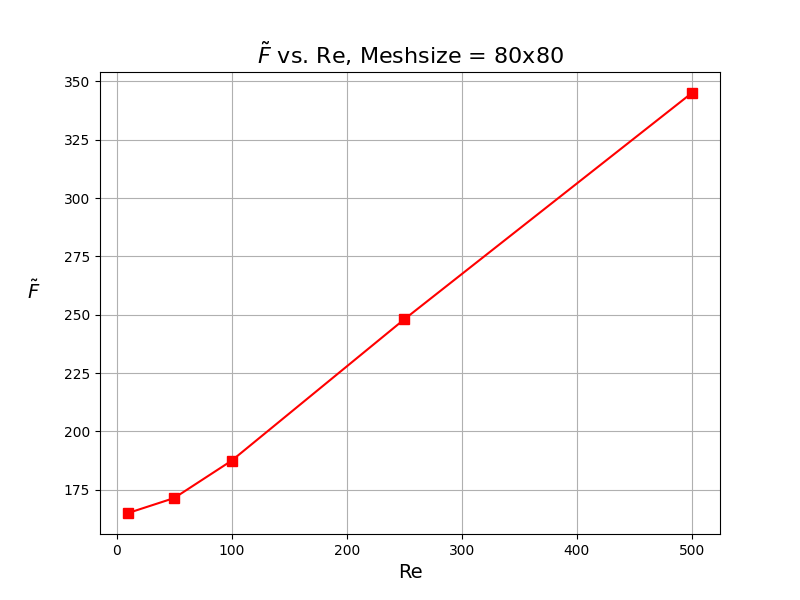
\includegraphics[width = \textwidth]{images/Nondimensional_Force_vs._Re.png}
   \caption{Force increases with higher Reynolds flow}
   \label{force}
\end{figure}

The trapezoidal method of integration,
\begin{equation*}
   \displaystyle \int_{0}^{1} \tilde{\tau}(\tilde{x})\, d\tilde{x} = \sum_{i=0}^{80} \dfrac{\tilde{\tau}_{i}+\tilde{\tau}_{i+1}}{2} \Delta{\tilde{x}}
\end{equation*}

where $\Delta{\tilde{x}} = \frac{1}{80}$.


\pagebreak
\appendix
\pagenumbering{gobble} 
\begin{center}
\vspace*{\fill}
   \Huge \bf Appendix 
\vspace*{\fill}
\end{center}
\pagebreak 

\hypertarget{code}{}
\section{Code}
PDF of code starts on next page. 
\vspace{2.5mm}

Additionally, team repository: \url{https://github.com/andressuniaga/CFD-SP25-11}

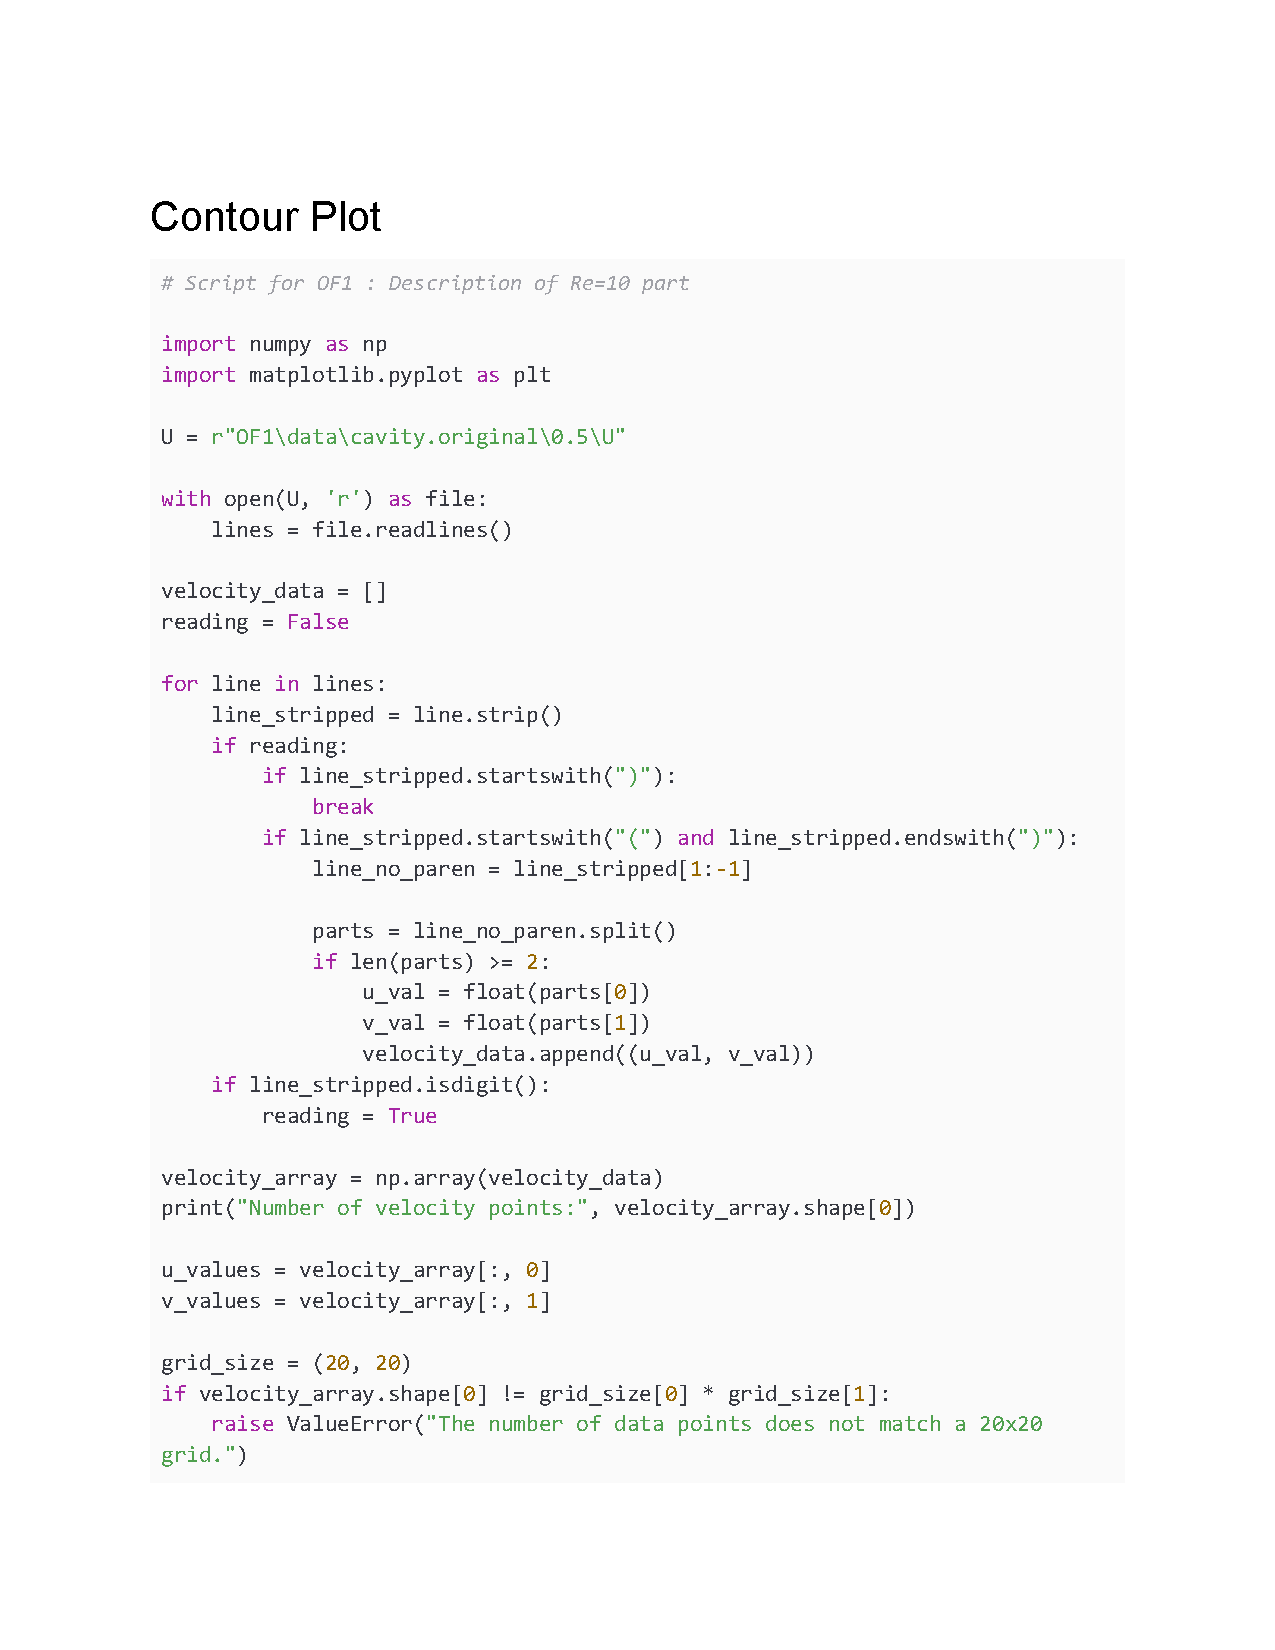
\includepdf[pages=-]{CFD OF1 Code.pdf}

\end{document}